%-----------------------------------------------------------------
%Esta será la presentación de nuestra Aplicación.
%-----------------------------------------------------------------

\documentclass{article}

%-------------------------- Preámbulo -------------------------

% character encoding
\usepackage[utf8]{inputenc}                   % replace by the encoding you are using
\usepackage{graphicx} % Required to insert images

%-------------------- Empieza el document -------------------

\begin{document}

\title{Aplicación para Android\\FindMe}
\author{Stella Andrade\\Danny Ponce\\Kevin Silva}
\date{}
\maketitle

\section{Características generales}
FindMe es una aplicación que actúa como un botón de pánico: al llegar a una zona peligrosa, se activaría la aplicación -la cual actuará en segundo plano- y la aplicación empezará a enviar mensajes al correo electrónico guardado cada cierto tiempo, con la hora y la ubicación GPS del dispositivo.

La aplicación seguirá activada hasta que se la desactive presionando el botón para desactivarla e ingresando una contraseña registrada en el primer uso de la aplicación. Se enviará un mensaje al correo avisando que será el último mensaje 
\newpage
\section{Prototipo}
Un diseño muestra de cómo sería la aplicación.\\
\begin{center}
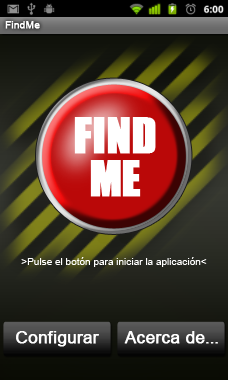
\includegraphics{findmesscreenmain}\\\emph{Prototipo de la pantalla principal de la aplicación FindMe}

\paragraph{Configurar}
Aquí podrá editar su información de contacto: correo electrónico principal, número de teléfono (opcional), cambiar la contraseña y el intervalo de tiempo de envio de los mensajes.
\paragraph{Acerca de...}
Aquí estará la información de la aplicación, número de versión y tal.
\end{center}

Pero al iniciar la apliación por primera vez, será recibido por otra pantalla donde debe ingresar las direcciones seguras, y asignar una contraseña.
\begin{center}
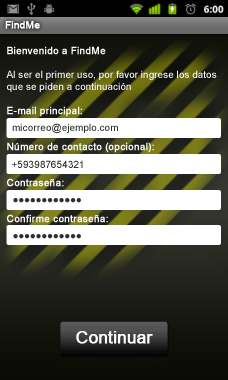
\includegraphics{findmefirstscreen}\\\emph{Pantalla al utilizar por primera vez la aplicación.}
\end{center}

Al estar activa la aplicación trabajará en segundo plano, pero al llamar a la aplicación luego aparece la ventana para desactivarlo, donde pide la contraseña.
\begin{center}
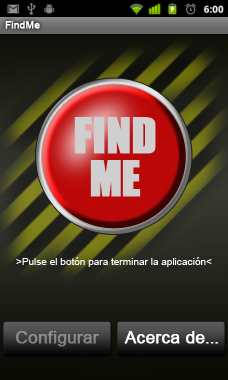
\includegraphics{findmesscreenfinal}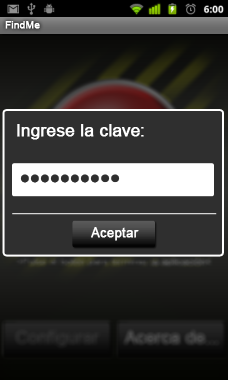
\includegraphics{findmesscreenfinal2}\\\emph{Pantalla al terminar de utilizar la aplicación.}
\end{center}

\newpage
\section{Experiencia con el proyecto}

Para la realización de este proyecto tuvimos que usar herramientas que nunca habíamos usado antes: \LaTeX{} y GitHub, sin contar con la IDE dirigida a las aplicaciones móbiles.

El uso de \LaTeX{} realmente fue muy complicado; buscar los comandos necesarios para que hagan las cosas que quisiéramos, la sintaxis, las incompatibilidades y la falta de algunas librerías (como la de Beamer al principio).

Con GitHub también se nos complicó un poco, con la creación de llaves y adaptarnos al shell estilo Linux para hacer los commits, y ahora con lo que debemos trabajar distintas cuentas colaborando (aún estamos probando esa característica).

Ambas herramientas son muy útiles, pero hay que dedicarle mucho tiempo a su uso y práctica para poderlos usar al máximo.

\end{document}